\documentclass[10pt,a4paper,oneside]{report}

\usepackage[section] {placeins}
\usepackage[dvipsnames]{xcolor}
\usepackage{graphicx} % in order to insert images
\usepackage{tabularx}
\usepackage[headings]{fullpage} % wider
\usepackage{verbatim} % enable verbatim text for code etc.
\usepackage{caption}
\usepackage{minitoc}
% \usepackage{cite} % we want to cite our bibliography
\usepackage{natbib} % citep used when author-date citation styles are required?
\usepackage{fancyhdr}
\usepackage{enumerate} % we want lists.
\usepackage{enumitem} % less gap between items
\usepackage{soul}
\usepackage{amsmath} % math symbols
\usepackage{listings}
\usepackage{tablefootnote} % for handling footnote in tables
\usepackage{float} % for placing figures/tables at the specified place in text with [H]
\usepackage[linkcolor={blue},citecolor={blue},urlcolor={red}]{hyperref}

% Package configutations
\newcommand{\notimplies}{\mathrel{{\ooalign{\hidewidth$\not\phantom{=}$\hidewidth\cr$\implies$}}}}
\newcommand{\HRule}{\rule{\linewidth}{0.5mm}} % Header
\lstset{basicstyle=\ttfamily\footnotesize,breaklines=true,aboveskip=25pt,belowskip=25pt} % code box
\hypersetup{urlcolor=blue, colorlinks=true} % Colors hyperlinks in blue

% Custom variables
\def \thesistitle{Our awesome title}
\def \authorname{Thomas Almenningen, Martin Christian Havig and Herman Schistad}
\def \supheri{Heri Ramampiaro}
\def \suphelge{Helge Langseth}
\def \degreename{Computer Science}
\def \groupname{Artificial Intelligence Group}
\def \deptname{IDI}

% PDF-metadata
\hypersetup{pdftitle={\thesistitle}}
\hypersetup{pdfauthor=\authorname}

\begin{document}

%----------------------------------------------
% TITLE PAGE
%----------------------------------------------

\begin{titlepage}
\begin{center}
%\includegraphics[scale=1.1]{fig/rams}
\mbox{}\\[6pc]
\begin{center}
\Huge{\thesistitle}\\[2pc]

\Large{\authorname}\\[1pc]
\large{\today}\\[2pc]

MASTER THESIS\\
Department of Computer and Information Science\\
Norwegian University of Science and Technology
\end{center}
\vfill

\noindent Supervisor: \supheri \\
\noindent Supervisor: \suphelge

	%{\Huge Twilm} \\
	%\medskip
  %  \vspace{\stretch{0.2}}
%
 %   { \Large \bfseries PROJECT}
  %  \HRule \\[0.5cm]
	%{ \huge \bfseries ONELINER ABOUT \\[0.4cm]}

   % \HRule \\[0.5cm]

   % \begin{minipage}{0.4\textwidth}
   %     \begin{flushleft} \large
   %         \emph{Authors}\\
   %         Martin Christian \textsc{Havig} \\
   %     \end{flushleft}
   % \end{minipage}
   % \begin{minipage}{0.4\textwidth}
   %     \begin{flushright} \large
   %         \emph{Supervisor:} \\
   %         Some  \textsc{One}
   %     \end{flushright}
   % \end{minipage}

    %\vfill
   % \today \\\ \\\
\end{center}
\end{titlepage}

\clearpage

%----------------------------------------------
% ACKNOWLEDGEMENTS
%----------------------------------------------

\renewcommand{\abstractname}{Acknowledgments}
\begin{abstract}
\end{abstract}

%----------------------------------------------
% ABSTRACT
%----------------------------------------------

\renewcommand{\abstractname}{Abstract}
\begin{abstract}

\end{abstract}
\pagenumbering{roman}

%----------------------------------------------
% TABLE OF CONTENTS
%----------------------------------------------

\setcounter{tocdepth}{2}
\dominitoc
\minilof
\minilot
\tableofcontents
\clearpage
\listoffigures
\listoftables

\setcounter{tocdepth}{1}

%----------------------------------------------
% CHAPTERS
%----------------------------------------------

% !TEX root = ../report.tex

\chapter{Introduction}
\label{chap:introduction}
\minitoc
\setcounter{page}{1}
\pagenumbering{arabic}
\clearpage

\newcommand{\ecommercenorway}[0]{
  \begin{figure}[H]
    \centering
    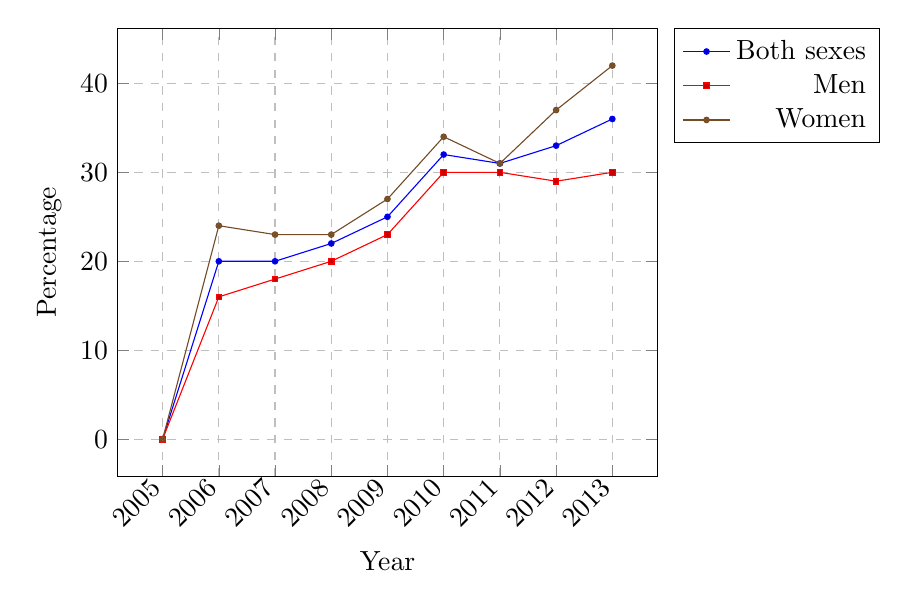
\begin{tikzpicture}
      \begin{axis}[
        xlabel={Year},
        ylabel={Percentage},
        legend style={cells={anchor=east}, legend pos=outer north east,},
        xtick=data,
        x tick label style={rotate=45, anchor=east, /pgf/number format/1000 sep=},
        mark size=1.0pt,
        grid=major,
        grid style={dashed},
      ]
      \legend{Both sexes, Men, Women}
      \addplot coordinates {
        (2005, 0)
        (2006, 20)
        (2007, 20)
        (2008, 22)
        (2009, 25)
        (2010, 32)
        (2011, 31)
        (2012, 33)
        (2013, 36)
      };
      \addplot coordinates {
        (2005, 0)
        (2006, 16)
        (2007, 18)
        (2008, 20)
        (2009, 23)
        (2010, 30)
        (2011, 30)
        (2012, 29)
        (2013, 30)
      };
      \addplot coordinates {
        (2005, 0)
        (2006, 24)
        (2007, 23)
        (2008, 23)
        (2009, 27)
        (2010, 34)
        (2011, 31)
        (2012, 37)
        (2013, 42)
      };
      \end{axis}
    \end{tikzpicture}
    \label{fig:ecommerce-in-norway}
    \caption{E-commerce purchases in Norway since 2005~\cite{statisticsNorway}}
  \end{figure}
}

\section{Motivation}
\label{sec:motivation}

% What are recommender systems good for?
In today's day and age the increasing amount of data overwhelm our human
processing capabilities in many information seeking tasks. To cope with this
overload researchers have introduced recommender system to filter the ever
increasing information and only present a small selection of items which
reflects the users tastes, interests and priorities. Recommender systems are an
active research field and has been successfully applied to many different
services ranging from e-commerce sites such as \emph{Amazon}, movie and
TV-series streaming services like \emph{Netflix} and in different music
applications such as \emph{Last.fm} and \emph{iTunes}.

% What is telenors incentive?
Many of the largest commerce Web sites have been using recommender systems to
help their customers find products to purchase for nearly two decades.
Schafer et al.~\cite{Schafer1999} identified three ways, in which recommender
systems increase E-commerce sales: (1) Browser into buyers: Recommender systems
can help customers find products they wish to purchase, (2) Cross-sell:
Recommender systems improve cross-sell by suggesting additional products for
the customer to purchase and (3) Loyalty: In a world where the competitor only
is one click away, gaining customer loyalty is an essential customer strategy.
Recommender systems improve loyalty by creating a value added relationship
between the site and the customer.

% What is the app and what makes it unique?
SoBazaar is a new \textit{fashion e-commerce application} for web and hand held
devices developed by Telenor, Norway's largest Telco company. The application
aggregates fashion products from various brands and stores into one \emph{news
feed} with recommended products, enabling the user to shop clothes and
accessories effortlessly and without the need of registering an account on
multiple web stores. Currently the application makes global recommendations
based on popular products and trends within social networks --- however, the goal
before launching the application this upcoming summer (\the\year) is to improve
these ratings making them personalized and grounded in a larger array of
features. This has as noted the potential of improving sales, activity and user
satisfaction.

% Discuss potential in fashion and e-commerce sales.
\ecommercenorway{}

The growth potential of such an application is immense in Norway. Numbers from
Statistics Norway~\cite{statisticsNorway} which are presented in the above
figure, shows a steady increase in the number of e-commerce sales of about 8\%
per year, from 2005. Still the competition, especially within personalized
recommendations, is insubstatial at both a national and international level, as
we will see in a detailed comptetitor analysis in
Section~\ref{subsec:competitors}. This underlines the importance of both the
discoveries made in this thesis and the application itself.

% Limited amount of data -> we need to utilize other sources. Implicit!
As the application is not yet officially released there is a limited amount of
user-item interaction from a set of beta users. In addition users do not have
the possibility to explicitly rate items on a numeric scale, a scheme often
employed by machine learning engineers and application developers in order to
understand their users preferences. Combining these two factors makes the
recommendation scenario both interesting and unique, since we need to utilize
the implicit information contained in user behavior such as clicking, wanting
or buying an item. Limited data both in number of users, but also in activity,
makes the system prone to what is called \textit{cold-start issues}, where
making recommendations with limited information is resolved by a variety of
techniques.

% The fashion domain have certain challenges.
This scenario differs from making recommendations on movies, books and music,
not just in the lack of rich explicit ratings, but also in the context of the
domain the recommendations will be done, namely the fashion domain. Firstly,
fashion consumption is largely determined by seasons. E.g. one does not buy
winter jackets in the middle of summer. Most clothes do also go out of
fashion, the same can not be said for \emph{all} movies. Secondly, there are a
whole different set of important aspects regarding the items or products when
recommending in the fashion domain, such as: brand, color and size.

% Brand and price are important!
Finally, users are highly price and brand-aware. This can be exemplified by
looking at an average movie consumer, where typically the director of the movie
does not greatly affect the way the movie is consumed. However, in the fashion
domain the consumer might mainly look at the product brand when deciding what
to consume. Price preferences are also related to this property where some
users prefer making \textit{a good deal} on periodic sales whilst other buys
clothes not only for individual satisfaction, but to show of or make a
statement.

% What are our goals and purpose?
In our system, there are two sources of information available for making
recommendations: an aggregated product database and event logs capturing user
activities. Out first goal is to find a technique for translating the implicit
feedback into preferences. These preferences are then combined with product
features and techniques for mitigating the cold-start problem. Finally the
user-item preferences are utilized in making recommendations where challenges
related to both domain and data sources are considered.

% Example scenario
For the users of SoBazaar the final product should not infer with the already
established user interface. Instead the news feed will evolve from today
showing the same recommendations to all users, to showing \textit{personalized
recommendations} to every user, based on their \textit{behavior} in the
application. For every user-item interaction the user is implicitly changing
his/hers preference-profile and will then, by just using the application, get
novel and more robust recommendations. Further, as personalized recommendations
hopefully will increase both sales and user activity we will, with a larger set
of data, be able to understand more user patterns and consequently gain a
deeper understanding of the domain.

\section{Problem Statement and Goals}

% Overall problem statement
The primary aim of this thesis is proposing a system, producing personalized
fashion recommendations based on user behaviour and product features, when both
resources are extremely limited in both quality and volume.

% Introduce goals related to domain
In order to propose such a system, one need a exhaustive understanding of both
the fashion domain and available data. In addition a study is required looking
at existing solutions, competitors and idientify potential competitive
advantages. Finally a discussion on how to overcome found challenges with
respect to both understanding the implicit feedback and making recommendations
is needed. Hence, our domain specific goals can be defined as:

% Domain-specific goals
\begin{itemize}
	\item \textbf{G1}: Gain a better understanding of the fashion domain.
  \item \textbf{G2}: Identify the specific challenges of making fashion recommendations.
  \item \textbf{G3}: Study how existing technologies can be adapted to mitigate or
  overcome these challenges.
\end{itemize}

% Introduce goals related to cold-start
In most recommender systems one base future recommendations on existing
feedback already given by the user. An important however is what to recommend
when no feedback has been given, which is the case for any new user. The same
issue is apparent when a new item is added to the application, where we need a
strategy for introducing it to users although the product is not connected to
any existing feedback. Finally, the closely related problem of making
recommendations in scenarios where feedback is extremely sparse need to be
addressed. First impressions are important both for retention and customer
satisfaction and consequently, seperate goals were set specifically concerning
cold-start issues.

\begin{itemize}
  \item \textbf{G4}: Study existing solutions to the cold-start.
  \item \textbf{G5}: Identify the best suited methods with regards to both application
  feedback and domain.
\end{itemize}

% Introduce goals related to implicit feedback
There is no explicit way for users to \textit{rate} or give \textit{negative
feedback} to items in SoBazaar. This forces us to look at user behaviour and
more specifically interactions on items such as \textit{clicking},
\textit{wanting} or \textit{purchasing}. We would like to learn how these
events could be used to predict the users true preferences. Using implicit
feedback yields the following goals:

\begin{itemize}
  \item \textbf{G6}: Explore the existing solutions of how to infer user preference from
  implicit feedback data.
  \item \textbf{G7}: Identify different methods of combining various event types into
  \emph{implicit ratings}.
  \item \textbf{G8}: Find metrics in order to evaluate the \emph{implicit ratings}.
\end{itemize}

% Introduce limitations
\paragraph{Limitiations} Our problem statement and consequent goals establish
the main theme of this thesis, but simultaneously they introduce some
limitiations. Hence, the reader should be familiar with what this thesis
\textit{does not set out to do}.

% Small and sparse dataset
The main limitiation of this thesis are primarly linked to having only one
available dataset with both sparse and modest data. As a result, making
conclusions based user behaviour proved difficult due to lack of statistical
significance on many observations. Limitiations in both time available and
number of existing users with sufficient activity made is also impossible to
conduct a thorough user study, which could confirm possible found user
patterns.

% No external sources of information (or weak quality)
In addition, as seen in the overview, external sources of information such as
social networks and trust-based networks are not considered --- as the dataset
provided did not warrant this. As the products in the SoBazaar application are
aggregated from multiple sources, and hence product databases, the quality of
information are notably diverse. Consequently, since extracting basic content
features different from product titles became close to impossible without large
engineering efforts, the \textit{main focus} does not lie on hybrid recommender
systems (combining content and user-based recommendations), although some work
is done in this area.

\section{Application Overview}

\begin{figure}[H]
  \centering
  \begin{tikzpicture}[
    % Manually overriden in most of the nodes :-)
    node distance=2.3cm,
    block/.style={
      rectangle,
      draw,
      thick,
      inner sep=5pt,
      align=center,
      rounded corners,
      minimum width=2cm,
    },
    % Special style for the social networks
    social/.style={
      draw=red,
      densely dotted,
    },
    % Box surrounding the data sources.
    dsbox/.style={
      draw,
      dotted,
      minimum height=1.2cm,
    }
  ]

  % Create nodes - first, data sources.
  \node(db)     [block] {Product DB};
  \node(social) [block,social, right of=db] {Social data};
  \node(log)    [block,right of=social] {Event log};

  % Our various 'systems'
  \node(coldstart) [block, below = 3.5cm of db] { Cold-start\\booster };
  \node(converter) [block, below = 3.5cm of log] { Implicit\\Converter };
  \node(recommender) [block, below = 2cm of coldstart] { Recommender };
  \node(evaluation) [block, right = 3.5cm of recommender] { Evaluation };

  % Box around data sources.
  \node (datasources) [dsbox, fit=(db) (social) (log)] {};
  \node at (datasources.north) [above, inner sep=2mm] {Data sources};

  % Draw the links between systems and data sources.
  \path[->,thick]
     (log) edge [] node [sloped, above] {Implicit feedback} (converter)
     (db) edge [] node [sloped, above, text width=3cm, align=center] {Structured\\product data} (coldstart)
     (converter) edge [] node [sloped, above] {Ratings} (coldstart)
     (coldstart) edge [] node [sloped, above] {Ratings} (recommender)
     (recommender) edge [] node [sloped, above] {Recommendations} (evaluation);

  \end{tikzpicture}
  \caption{Application overview, showing input and output from different
  components in the proposed system}
\end{figure}

\section{System Overview}

\marginpar{Include filterbots in a more detailed system overview?}

This thesis proposes a system for making recommendations based on implicit
data, where the input is implicit feedback collected on a set of users and
items and the output is personalized recommendations to all users, proposing
new and relevant products to their preferences.

\begin{figure}[H]
  \centering
  \begin{tikzpicture}
    [node distance = 1cm, auto,font=\footnotesize,
    % STYLES
    every node/.style={node distance=1.5cm},
    % The comment style is used to describe the characteristics of each process
    comment/.style={rectangle, inner sep= 5pt, text width=4cm, node distance=0.25cm, font=\scriptsize\sffamily},
    % The nonProcess style
    nonProcess/.style={rectangle, draw, inner sep=5pt, text width=4cm, text badly centered, minimum height=1.2cm, font=\footnotesize\sffamily},
    % The process style is used to draw the processs' name
    process/.style={rectangle, draw, fill=black!10, inner sep=5pt, text width=4cm, text badly centered, minimum height=1.2cm, font=\bfseries\footnotesize\sffamily}]

    % Draw processs
    \node [nonProcess] (inputData) {Input data based on implicit feedback (events)};
    \node [process, below of=inputData] (implicitConverter) {Convert implicit feedback to implicit ratings};
    \node [nonProcess, below of=implicitConverter] (ratings) {Ratings};
    \node [process, below of=ratings] (recommendations) {Recommending};

    \node [comment, right=0.25 of inputData] (comment-inputData) {
      Implicit Feedback (clicks, purhcases etc.) collected from the SoBazaar
      analytics logs. Detailed description in Section~\ref{sec:sobazaar-data}
    };

    \node [comment, right=0.25 of implicitConverter] (comment-implicitConverter) {
      Converts the inputed implicit feedback to implicit ratings based on
      different conversion schemes. Detailed description in
      Section~\ref{sec:implementation-implicit}
    };

    \node [comment, right=0.25 of ratings] (comment-ratings) {
      Set of rating triplets, on the form \textit{user, product, rating}.
    };

    \node [comment, right=0.25 of recommendations] (comment-recommendations) {
      Makes recommendations based on the inputed ratings. Different
      approaches to make the recommendations can be take, such as matrix
      factorization or neighborhood based approaches. Detailed description in
      Section~\ref{sec:making-recommendations}
    };

    % Draw the links between processs
    \path[->,thick]
      (inputData) edge (implicitConverter)
      (implicitConverter) edge (ratings)
      (ratings) edge (recommendations);

  \end{tikzpicture}
  \caption{Overview of the system. Boxes in white represents input and output
  data. Boxes in gray represents processes}
\end{figure}

Traditionally in most recommender systems this process does not include the
first two stages of our system, hence going directly from a set of explicitly
provided ratings to a set of recommendations. However, as we will see, making
ourselves non-dependent on explicit ratings can both provide us with a good
set of recommendations and take us one step closer to true artificial
intelligence, as we require no extra effort from the users --- rather learning
preferences from their behavior.

\section{Outline}
\begin{table}[H]
  \centering
  \begin{tabular}{lp{11cm}}
  \toprule
    \textbf{Chapter}      & \textbf{Description} \\
  \midrule

    Chapter \ref{chap:introduction} & The~\nameref{chap:introduction} chapter gives an overview of the
    project to the reader. It also outlines the purpose and motivation of the
    project.  \\[1.5ex]

    Chapter \ref{chap:thesobazaardata} & \nameref{chap:thesobazaardata} chapter presents the results from our
    dataset analysis. \\[1.5ex]

    Chapter \ref{chap:SotA} & The \nameref{chap:SotA} chapter documents knowledge,
    research and technology that are relevant to the project, and how and why
    some of them were prioritized over others when it comes to how they are
    used in the project. \\[1.5ex]

    Chapter \ref{chap:implementaion} & The \nameref{chap:implementaion} chapter describes the design of the
    system and how the design has been implemented. \\[1.5ex]

    Chapter \ref{chap:resulteval} & The \nameref{chap:resulteval} chapter discus the development process,
    testing of results and major issues. \\[1.5ex]

    Chapter \ref{chap:conclusion} & The \nameref{chap:conclusion} chapter sums up the project and describes the
    findings and reflects on them. It also describes further work.
    \\[1.5ex]

    Appendix & \textbf{The Appendix} contains extended information such as a full list of the requirements. \\

  \bottomrule
  \end{tabular}
  \caption{Overview of structure and chapters in the thesis}
  \label{table-reportstructure}
\end{table}

% !TEX root = ../report.tex

\chapter{Preliminary Study}
\minitoc

\clearpage

\section{State Of The Art}
\subsection{System Coldstart Handling}
\subsection{Fashion Recommendation}
\subsection{Session Based Recommendation}
Articles 4 l8er:
In Proceedings Of
the 1995 International Joint Conference on Artificial Intelligence, 1995. Montreal,
Canada.

S. Schechter, M. Krishnan, and M. D. Smith. Using path profiles to predict http
requests. In Proceedings of 7th International World Wide Web Conference, Novem-
ber 1998. Brisbane, Australia.

M. Spiliopoulou and L. C. Faulstich. Wum: A web utilization miner. In In Pro-
ceedings of EDBT Workshop WebDB98, 1999. Valencia, Spain.

R. Cooley, B. Mobasher, and J. Srivastava. Data preparation for mining world wide
web browsing patterns. Journal of Knowledge and Information Systems, 1(1), 1999.

B. Mobasher, H. Dai, T. Luo, and M. Nakagawa. Discovery of aggregate usage
profiles for web personalization. In Proceedings of the Web Mining for E-Commerce
Workshop (WebKDD’2000), 2000.

C. Shahabi, A. Zarkesh, J. Adibi, and V. Shah. Knowledge discovery from users
web-page navigation. In Proceeding of the IEEE RIDE97 Workshop, pages 20–29,
April 1997. Birmingham, England.

O. Nasraoui, R. Krishnapuram, and A. Joshi. Mining web access logs using a fuzzy
relational clustering algorithm based on a robust estimator. In Proceedings of Eight
International World Wide Web Conference, 1999. Toronto, Canada.

Y. Yan, M. Jacobsen, Garc ̈ıa-Molina H, and U. Dayal. From user access patterns to
dynamic hypertext linking. In Proceedings of the Fifth International World Wide
Web Conference, 1996. Paris, France.

A. Nanopoulos, D. Katsaros, and Y. Manolopoulos. Effective prediction of web-
user accesses: a data mining approach. In Proceedings of WEBKDD workshop,
2001. San Francisco, CA, USA.

R. Agrawal and R. Srikant. Mining sequential patterns. In Proceedings of the In-
ternational Conference on Data Engineering (ICDE), March 1995. Taipei, Taiwan

M. Deshpande and G. Karypis. Selective markov models for predicting web-page
accesses. In Proceedings of the First SIAM International Conference on Data Min-
ing (SDM’2001), 2001.

R. R. Sarukkai. Link prediction and path analysis using markov chains. In Proceed-
ings of the Ninth International World Wide Web Conference, 2000. Amsterdam.


%http://dl.acm.org/citation.cfm?id=1136004
%http://link.springer.com/chapter/10.1007/3-540-46119-1_42
%http://dl.acm.org/citation.cfm?id=1082567
%http://link.springer.com/chapter/10.1007%2F978-3-540-30214-8_20
%http://dl.acm.org/citation.cfm?id=502935
%http://dl.acm.org/citation.cfm?id=1835896
%http://dl.acm.org/citation.cfm?id=345169
%http://dl.acm.org/citation.cfm?id=345169

\subsection{Recommenders (Similar systems? somethingsomething)}

\section{Data Findings}
\subsection{What Can Be Understood From The Data}
\subsubsection{The Expected}
Event "app_started"; all have user_id's
Event "app_first_started"; all user_id's are NULL
Event "user_logged_in"; all have user_id's... (assigned with login, event saved after login?)

\subsubsection{The Strange}
NULL valued events: (Not all strange, but put together for readability)
facebook_share_changed
collection_viewed
wantlist_menu_entry_clicked
app_became_active

app_first_started
facebook_login_failed

> db.prod.distinct('event_json.ipAddress').length
9033
> db.prod.distinct('event_json.eventData.device_id').length
2644
> db.prod.distinct('user_id').length
1660

More devices than users, can't fill the blanks with device_id

\subsection{Graphs N' Shit}

\section{What to use}
\subsection{Some Awesome Algorithms (Build up with project progress)}
\subsubsection{The Good}
\subsubsection{The Bad}
\subsection{Why Not To Use These (Same As above)}
\subsubsection{The Good}
\subsubsection{The Bad}

\section{How to evaluate}
\subsection{What Has Been Done Before}
\subsection{What To Use}
\subsubsection{The Good}
\subsubsection{The Bad}

\section{Evaluation}

% !TEX root = ../report.tex

\chapter{Requirements}
\minitoc

\clearpage

\section{Capturing the Requirements}

\section{Functional Requirements}\label{section:functional-requirements}
\begin{description}
  \item[FR1]
  \item[FR6]
  \item[FR7]
\end{description}

\subsubsection{FR1}

\subsubsection{FR6}

\subsubsection{FR7}


\section{Non Functional Requirements}\label{section:non-functional-requirements}
\begin{description}
  \item[NFR1]
\end{description}

\subsubsection{NFR1}


\section{Prioritized Requirements}

% !TEX root = ../report.tex
\label{design}
\chapter{Design}
\minitoc 

\clearpage

\section{Architecture}

\subsection{Logical View}

\subsection{Process View}

\subsection{Physical View}

\section{Algorithm Design}

\subsection{Prediction}\label{algorithm-design:prediction}

% !TEX root = ../report.tex

\chapter{Implementation}
\minitoc

\clearpage

% !TEX root = ../../report.tex

\section{Generating implicit ratings}
\label{implementation-implicit}

In this section we continue solving the problem of generating ratings based on
implicit feedback found in analytics logs, as defined in
Section~\ref{implicit-feedback}. Our goal is two-fold:

\begin{itemize}
  \item Find novel ways of creating implicit ratings, remedying as many
  weaknesses and challenges, depicted in Section~\ref{implicit-weaknesses}, as
  possible
  \item Customize existing and new algorithms to our fashion domain, described
  in Section~\ref{motivation}
\end{itemize}

But first, we need a clear insight into evaluation of generated ratings –
as this will guide our choice of methods and give us clear metrics for
comparison of various techniques.

\subsection{Evaluating generated ratings}

The most important factor when creating ratings is to understand which implicit
data are available and what they mean and imply. When ratings are not explicit,
the implicit ratings becomes the recommender systems equivelent of a ground
truth and all later stages in the recommender pipeline (See Section~\ref{}) are
dependent on the ratings representing a users preferences.  Hence, when
evaluating conversion methods we can do an initial analysis without any metrics
by answering \textit{«Given our data, does this generalization make sense?»}.

As a good example we our fashion store, SoBazaar, but any other e-commerce
application is applicable. The naive way of creating implicit ratings in such a
domain would be to count the number of times the user clicked on an item, and
draw the conclusion that the higher number of clicks equalled a higher rating.
However, 

\subsection{Levels of frequency, with global popularity}
\ref{levels-frequency}

Considering the weaknesses presented in Section~\ref{levels-frequency}, namely
choosing good weights and only using a small percentage of the scale between
0-100. Further, the method presented does not differentiate between active and
less active users, thus ignoring the entropy once the maximal level is reached.
Instead we extend the method by considering the global popularity of each item,
so that the user that.. \marginpar{Finish the subsection about improving leveled
freq}

\subsection{Introduction to the sigmoid-function}

Extending our models further we want to capture our intuition that recent
events should count more towards a good rating, compared to old events. We
differentiate between two ways of classifying an event $e_u$ as old or recent;
one where we count the number of days between the newest event $e_n$ and event
$e_u$; and the second where we count the number of other events between $e_n$
and $e_u$. However, intuitively we consider a user to have multiple relevant
items concurrently and we know that in domains such as technology, fashion and
other consumer-products an item has an age of relevancy, somewhat metaphoric to
a seasonal threshold. An example of this could be a fashion store recommending
warm clothes in the months between December to March, but then want to "change"
product pool based on the users behaviours – who are probably looking for
lighter clothes (changing season).

By considering recentness we also implicitly add negative feedback to events,
as in practice we are penalizing the ratings for old events. This is an
important aspect to keep in mind when working with implicit feedback, as
discussed in Section~\ref{implicit-feedback} as modern recommender engines work
better when we are assuming ratings are based on both positive and negative
feedback.

In order to catch our intuition mathematically we use a logistic function, which
is a mathematical function having an "S" shape and a common special case of the
more general sigmoid-function. In its most simplest case the logistic function
is defined as:

% Vertical alignment of equation and plot.
\begin{figure}[H]
  \centering
  \noindent\begin{minipage}{.45\textwidth}
    \begin{tikzpicture}
      \begin{axis}
      \addplot[black,xlabel=$x$,ylabel=$f(x)$] {1/(1+exp(-x))};
      \end{axis}
    \end{tikzpicture}
  \end{minipage}
  \begin{minipage}{.45\textwidth}
  \begin{align}
    \label{logistic-function}
    f(x) = \frac{1}{1+\exp^{-x}}
  \end{align}
  \end{minipage}
  \caption{Logistic function having a S-shape with y-values ranging
  from 0 to 1.}
\end{figure}

Here the value of $f(x)$ is asymptotically limited between 0 and 1, dependent
on the value of $x$. The steepest point of the curve happens when $x=0$. By
adjusting the exponent of $e^{(-x)}$ we can skew the curve in order to map to our
data, giving us a \textit{function of relevancy} ranging from an item being
very relevant ($f(x)=0$) and not relevant ($f(x)=1$).

By adding two variables to the logistic function we can fine tune both the
steepness and range of $f(x)$. Hence we adjust Equation~\ref{logistic-function}
to include $s$, the \textit{steepness coefficient}, and $r$, the \textit{shift
coefficient}. By default these are $1$ and $0$ respectively, but by adjusting
$s$ closer to 0 we decrease the steepness, creating a more gradual curve.
Setting the $r$ to a larger number we shift the steepest point of the curve to
$x=r$, hence if we set $r$ to $20$, the steepest point (largest acceleration)
in our curve would be located when $x=20$.
\marginpar{show equation using these coefficients}

\subsection{Considering number of days since event}

In order to better understand the usage of the logistic function, we consider
an example event log.
%We are considering the following event log for user $u$ on product $p$, where
%our goal is to give a implicit rating based on different event types and the
%number of days between events.

\begin{table}[H]
  \centering
  \label{events-example}
  \begin{tabular}{p{4cm}m{3cm}}
    \toprule
    Number of days since most recent event & Unique event types \\
    \midrule
    5 & 1,2,3 \\
    10 & 1 \\
    15 & 1,2 \\
    \bottomrule
  \end{tabular}
\end{table}

As discussed in Section~\ref{implicit-feedback} and
Section~\ref{levels-frequency} we will use levels of frequency to order or
event types by scores, or rather importance. But, instead of sampling scores
between a given range we use a interval start and stop value - and use the
whole range of float values in this interval as possible scores. We can
imagine, for the purpose of this example that we have the following score
intervals:

\begin{table}[H]
  \centering
  \begin{tabular}{lll}
    \toprule
    Event type & Min. score & Max. score \\
    \midrule
    1 & 20 & 60 \\
    2 & 60 & 80 \\
    3 & 80 & 100 \\
    \bottomrule
  \end{tabular}
  \caption{Example of a scoring scheme using continious scores between a min.
  and max value as possible implicit scores}
  \label{implicit-example-scores}
\end{table}

\marginpar{\textbf{todo}: do evaluation on different schemes}
As discussed earlier, the way we assign these scores is at the moment fairly
naive, some results using various schemes are given in Section~\ref{}. The main
thing to note is that we use non-overlapping intervals in order to do various
optimizations in our algorithms and also that the interval for the most common
event (typically a product click or similar) is $3x$ as big as our higher
valued event types. This is done in order to create a larger differentiation
of scores between events of same type in the same time space.

Using the events in Table~\ref{events-example} we set our shift coefficient $r$
to $14.0$, and the steepness coefficient $s$ to $0.4$ in order to both match
our domain specific goals (short life span of products and seasonal activity)
and get a good spread in final ratings as our dataset is small. This yields the
following logistic function:

\begin{figure}[h!]
  \centering
  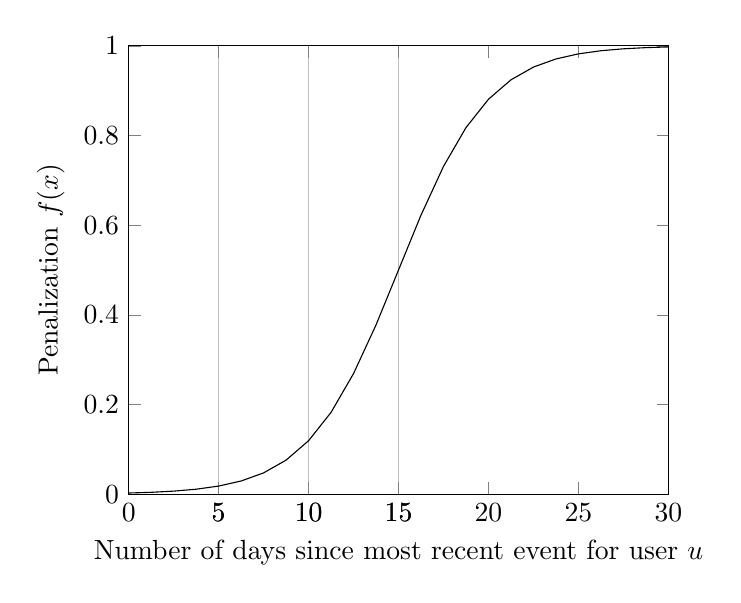
\begin{tikzpicture}
    \begin{axis}[
      ymin=0,ymax=1,
      xmin=0,xmax=30,
      xlabel=Number of days since most recent event for user $u$,
      ylabel=Penalization $f(x)$,
      extra x ticks={5,10,15},
      extra tick style={grid=major}
    ]
    \addplot[
    black,
    xlabel=$x$,
    ylabel=$f(x)$,
    domain=0:30]
    {1/(1+exp(-0.4*(x-15)))};
    \end{axis}
  \end{tikzpicture}
\end{figure}

As one can see, an event happening 15 days after the most recent event for user
$u$ will get a penalization of $0.5$ whilst an event with $x=5$ recieves
$0.018$. Following up on Table~\ref{events-example} we can calculate the
various penalizations and final scores for each day, by taking the highest
possible score for event $i$ and penalizing it in the following manner:

\begin{equation}
  s_{e}(x,u) = b_e - (b_e - w_e) \cdot p_{x}(u)
\end{equation}

where $p_x$ is the penalization after $x$ days. $b_e$ and $w_e$ are the best
and worst scores achievable for event $e$, respectivly. The final score
$s_{e}(x,u)$ is presented for each event below:

\begin{table}[H]
  \centering
  \begin{tabular}{llm{2cm}ll}
    \toprule
    Num. days ($x$) & Event types & Penalization $p_{x}(u)$ & Scores & Highest score \\
    \midrule
    5   & 1,2,3 & 0.018   & 59.1, 79.64, 99.64 & \textbf{99.64} \\
    10  & 1     & 0.1192  & 55.23              & 55.23  \\
    15  & 1,2   & 0.5     & 50.0, 70.0         & 70.0 \\
    \bottomrule
  \end{tabular}
  \caption[]{}
  \label{events-example}
\end{table}
\marginpar{Perhaps represent this differently?}

When selecting a score for user $u$ we select the highest valued one, in this
case 99.64. In fact, we can optimize our algorithm by starting at the most
recent events and not calculating scores for events types that yield a lower
score than the current highest score. In the scenario above we could take all
events on $x=5$, then taken the event type with highest maximum value (3) and
ignored all other events. Note that this is only true if you have
non-overlapping event type scores/intervals, as we have per
Table~\ref{implicit-example-scores}. We can now normalize $s$ and get a rating
$r$ between $a$ and $b$ by using the following equation, knowing that $X_{max}
= 100$ and $X_{min} = 0$:

\begin{equation}
  X' = a + \frac{(X-X_{min})\cdot(b-a)}{X_{max}-X_{min}}
  \label{eq-normalization}
\end{equation}

Setting $a$ to 0 and $b$ to 5, as is common in recommender systems we get the
rating $X' = 4.982$ when $s = 99.64$. Intuitivly this makes sense, if we assume
event type 3 to be the highest valued event in our system it would be
equivalaent to a user buying a product - or similar. Thus, if user $u$ bought
product $i$ only $5$ days ago this would get $4.98$ as final rating. If the
user does not interact with the product again in 30 days we can re-calculate
the score, now using $x=35$ which yields a penalization of $0.999$ and score $s
= 100-((100-80)*0,999) = 80.2$, normalized in the same likert scale as above we
get a new normalized rating $4.01$ - thus still a high rating, but not as
relevant for the user as 30 days earlier.

\subsection{Considering ordering of events}

In the our previous method using the number of days since the most recent event
we encounter several weaknesses when a user is either very active or have
events with a high degree of sparsity. In the latter a user interacting with
products every 20th day would see a divide in ratings since old events are
placed after at the top of the S-curve ($f(x) > 0.9$) and new events achieves a
penalization in the lower values ($f(x) < 0.1$). Similarily, when the user is
highly active we obtain a large number of items having the same penalization
weights and in essence a large duplication of ratings, provided the spread of
event types are not large, which in many systems are unlikely. One possibility
would be to use a finer granularity on the x values, such as seconds or minutes
since the most recent event, but instead we extend our method by not taking
into consideration the \textit{time}, but instead the \textit{ordering} of
events.

As before we use an example event log where we have 10 events of three
different types (1,2 and 3) on 6 different item IDs (1001-1006).

\begin{table}
  \centering
  \label{event-log-sigmoid-count}
  \begin{tabular}{lll}
    \toprule
    Ordering & Event type & Item id \\
    \midrule
    0 & 1 & 1001 \\
    1 & 1 & 1003 \\
    2 & 3 & 1002 \\
    3 & 1 & 1004 \\
    4 & 2 & 1002 \\
    5 & 2 & 1006 \\
    6 & 1 & 1005 \\
    7 & 1 & 1001 \\
    8 & 3 & 1005 \\
    9 & 1 & 1003 \\
    \bottomrule
  \end{tabular}
\end{table}

We want to continue using the sigmoid function, but in this case we will
differentiate based on how many events we observe for a user. Further, if a
user has e.g. more than 100 events in the event log we have two options: we can
set a ceiling, saying that events older than a threshold recieves the maximum
penalty or we can distribute all items evenly and extend the max-value of
x-axis. Probably one would want a combination of the two, having a pretty large
threshold and evenly distribute the items. In the case of evenly distribute the
values you would need a \textit{distribution factor} $f$ expressing the
relationship between steepness and shift coefficients. We use the following
equation where $c$ is the number of events for user $u$.

\begin{equation}
  f_{u}(x, c) =
    \begin{cases}
      1               & \text{if } c > 1000 \\
      \frac{1}{1+e^{-(f/c) \cdot (x - c)}} & \text{else }
    \end{cases}
\end{equation}

\subsection{Linearly blending the results}

\marginpar{Move this introduction to the pre-study?}
At this point we have found multiple novel ways of calculating the
implicit ratings, based on our implicit feedback. However, as one may observe
each method has its weknesses and strengths. A sigmoid-function considering the
number of days between events is good for including our implicit knowledge
about seasons into the ratings, but is not as effective if users has high
spread in between events or low activity. Further, there may exist some clothes
that has longer life-span than others, e.g. warm jackets that generally are
bought from September to March (7 months) compared to shorts which are
generally bought from May to August (4 months), depending on where the store
reside. Our second sigmoid function has the strength of always keeping the
ratings for a user fresh, also for less active users, but it is weaker in
differentiating between seasons - which can be seen if a user is on a hiatus
between January and August, not using the application. Upon return all ratings
would be based on his/hers winter activity, not penalizing the fact that the
type of clothes generally bought in the store at this time are different than
in January.

Optimally we would like to combine these two methods, taking their strenghts
and weaknesses together trying to average them out in order to end up with
generally better ratings - where we cannot trivally imagine scenarios as
depicted above where our models would fail. The process of combining such
ratings are in the Recommender Systems community called \textbf{blending} and
is in many ways a seperate research area in itself, if done advanced enough.
However, in the case of the naive and linear blend on can achieve results a
magninute higher than for each method seperatly as seen in \ref{}
\marginpar{find some refs using linear blending}.

When linearly blending $M$ models $m$, we choose $M$ factors $f$ all adding up
to 1.0, representing the weight of model $m_{i}$ in the final blend. Then when
calculating the final rating for item $j$ we sum over all models:

\begin{equation}
  r_j = \sum _{i=1}^{M} f_{i} * m_{j}
\end{equation}

As one may observe given the linear blend between with factors $f_1 = 0.7$ and
$f_2 = 0.3$ and the two ratings $m_1 = 5$ and $m_2 = 3$ for a given item, we
can calculate the final rating as $0.7 \cdot 5 + 0.3 \cdot 3 = 4.4$. A weakness
when linearly blending models in this way is the need for manually finding good
weights for the $M$ factors. There exists methods where this given a good test
set can be done automatically, such as using Linear Regression or KNN blending.
Many other blending schemes exists as well, such as Binned Linear Regression,
Bagged Gradient Boosted Decision Tree (BGBDT), Neural Networks and Kernel Ridge
Regression Blending \cite{jahrer2010combining} \cite{toscher2009bigchaos}.

As we have multiple proposed models we present our results given various
evaluation metrics and combinations of weights. Note that when a model has the
weight 1.0 its equal to that the model has not been blended with any other
model, and is included in the table below as a baseline.

\begin{table}[H]
  \centering
  \begin{tabular}{lll|ll}
    \toprule
    \textbf{Naive} &  \textbf{Sigmoid Count} & \textbf{Sigmoid Recent} &
    \textbf{RMSE} & \textbf{MAE} \\
    \midrule
    1.0  &      0.0        &      0.0       &  X   &  X  \\
    0.0  &      1.0        &      0.0       &  X   &  X  \\
    0.0  &      0.0        &      1.0       &  X   &  X  \\
    \midrule
    0.6  &      0.2        &      0.2       &  X   &  X  \\
    0.5  &      0.3        &      0.2       &  X   &  X  \\
    0.4  &      0.3        &      0.3       &  X   &  X  \\
    0.3  &      0.3        &      0.4       &  X   &  X  \\
    0.2  &      0.4        &      0.4       &  X   &  X  \\
    0.1  &      0.4        &      0.5       &  X   &  X  \\
    0.0  &      0.5        &      0.5       &  X   &  X  \\
    \bottomrule
  \end{tabular}
\end{table}

As one may see, the best results are achivied when blending with...
\marginpar{todo: analyze and finish this table}



% !TEX root = ../report.tex

\chapter{Evaluation}
\minitoc

\clearpage

\section{Development Process}

\subsection*{Good}

\subsection*{Bad}


\section{Result Evaluation}

\subsubsection{Testing of preliminary study}

\subsubsection{Testing of code functionality}

\subsubsection{Types of testing not used}


\section{Issues}\label{sec:issues}

% !TEX root = ../report.tex

\chapter{Conclusion}
\minitoc

\clearpage

\section{Final Product}


\section{Related Work}


\section{Future Work}


% !TEX root = ../report.tex

\appendix
\clearpage
\pagenumbering{Roman}
\setcounter{page}{1}

\chapter{Data}\label{app:req}
    \begin{table}[H]
        \centering
        \begin{tabular}{l|l}
            \toprule
            \emph{Variable}        & \emph{Example}   \\
            \midrule
            \emph{app\_version}   &   0.3  \\
            \emph{user\_agent}"   &   "SOBAZAR 0.3 (iPhone; iPhone OS 6.1.4; Scale/2.00; nb\_NO)"   \\
            \emph{product\_type}  &   "product"    \\
            \emph{server\_time\_stamp} &   "2013-10-24T11:33:17.632Z"   \\
            \emph{dy}    &   24   \\
            \emph{origin\_ui} &   "storefront"     \\
            \emph{currency}  &   "kr"     \\
            \emph{country\_name}  &   "Norway"     \\
            \emph{price} &   1995     \\
            \emph{product\_name}  &   "DWS No47"   \\
            \emph{tag\_name}  &   "NULL"   \\
            \emph{tag\_id}    &   "NULL"   \\
            \emph{storefront\_name}   &   "BIK BOK"    \\
            \emph{event\_id}  &   "product\_purchase\_intended"  \\
            \emph{age\_target}    &   "Any"    \\
            \emph{epoch\_day} &   16002    \\
            \emph{mo}    &   10   \\
            \emph{yr}    &   2013     \\
            \emph{product\_id}    &   2298002  \\
            \emph{event\_location}    &   Geo Location     \\
            \emph{ipAddress} &   IP  \\
            \emph{contentDescription}    &   null     \\
            \emph{sessionId} &   null     \\
            \emph{contentId} &   null     \\
            \emph{instKey}   &   "ed4c76251ac47da54299d8c0bce3dca6"   \\
            \emph{viewer}    &   null     \\
            \emph{ts}    &   NumberLong("1382614397632")  \\
            \emph{gender\_target} &   "Female"     \\
            \emph{client\_time\_stamp} &   "NULL"   \\
            \emph{login\_type}    &   "NULL"   \\
            \emph{transaction\_id}    &   "N/A"    \\
            \emph{service\_id}    &   "SOBAZAR"    \\
            \emph{platform}  &   "iPhone"     \\
            \emph{epoch\_week}    &   2286     \\
            \emph{storefront\_id} &   23002    \\
            \emph{hr}    &   11   \\
            \emph{tag\_position}  &   "NULL"   \\
            \emph{time\_stamp}    &   "2013-10-24T13:33+0200"  \\
            \emph{retailer\_brand}    &   13001    \\
            \emph{storefront\_position}   &   2    \\
            \emph{user\_id}   &   1342189870   \\
            \emph{country\_id}    &   194001   \\
            \emph{server\_environment}    &   "prod" \\
            \bottomrule
        \caption[Complete List of Event Metadata]{Table of the complete list of event metadata stored when an event is triggered}
        \label{table:completeEventData}
        \end{tabular}
    \end{table}

    \begin{table}[H]
        \centering
        \begin{tabular}{l}
            \toprule
            \emph{Event Name}   \\
            \midrule
            \emph{activity\_clicked}  \\
            \emph{storefront\_clicked}  \\
            \emph{product\_detail\_clicked}  \\
            \emph{user\_logged\_in}  \\
            \emph{featured\_collection\_clicked}  \\
            \emph{app\_started}  \\
            \emph{featured\_storefront\_clicked}  \\
            \emph{product\_wanted}  \\
            \emph{around\_me\_clicked}  \\
            \emph{menu\_opened}  \\
            \emph{end:app\_backgrounded}  \\
            \emph{app\_became\_active}  \\
            \emph{wantlist\_menu\_entry\_clicked}  \\
            \emph{content:interact:item\_scroll}  \\
            \emph{navigation:paging\_triggered}  \\
            \emph{content:explore:user\_logo\_clicked}  \\
            \emph{collection\_viewed}  \\
            \emph{stores\_map\_clicked}  \\
            \emph{product\_purchase\_intended}  \\
            \emph{friend\_invited}  \\
            \emph{store\_clicked}  \\
            \emph{facebook\_login\_failed}  \\
            \emph{end:app\_closed}  \\
            \emph{content:explore:search}  \\
            \emph{navigation:navbar:sobazaar\_icon}  \\
            \emph{app\_first\_started}  \\
            \bottomrule
        \caption[List of Different Events]{Table of the different events that can be triggered by the user and an explanation}
        \label{table:events}
        \end{tabular}
    \end{table}


    \begin{figure}[H]
        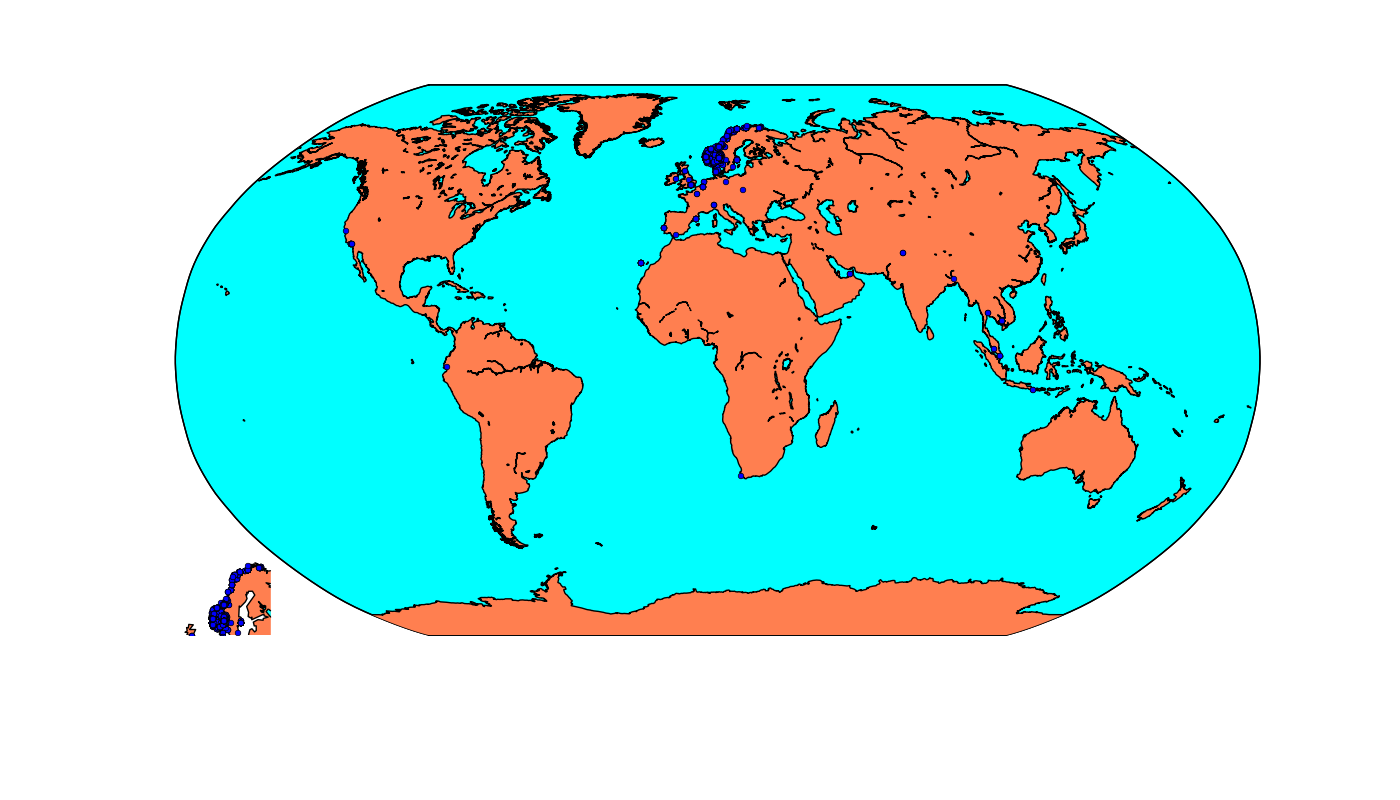
\includegraphics[width=5in]{image/simpleGeoPlotworld.png}
        \centering
        \caption[Event location mapped on the world]{This figure shows the location of the events from all over the world.
        For a cropped version with focus on Norway and the surrounding countries, refer to~\ref{figure:croppedGeoplot}}
    \end{figure}

    \begin{figure}[H]
        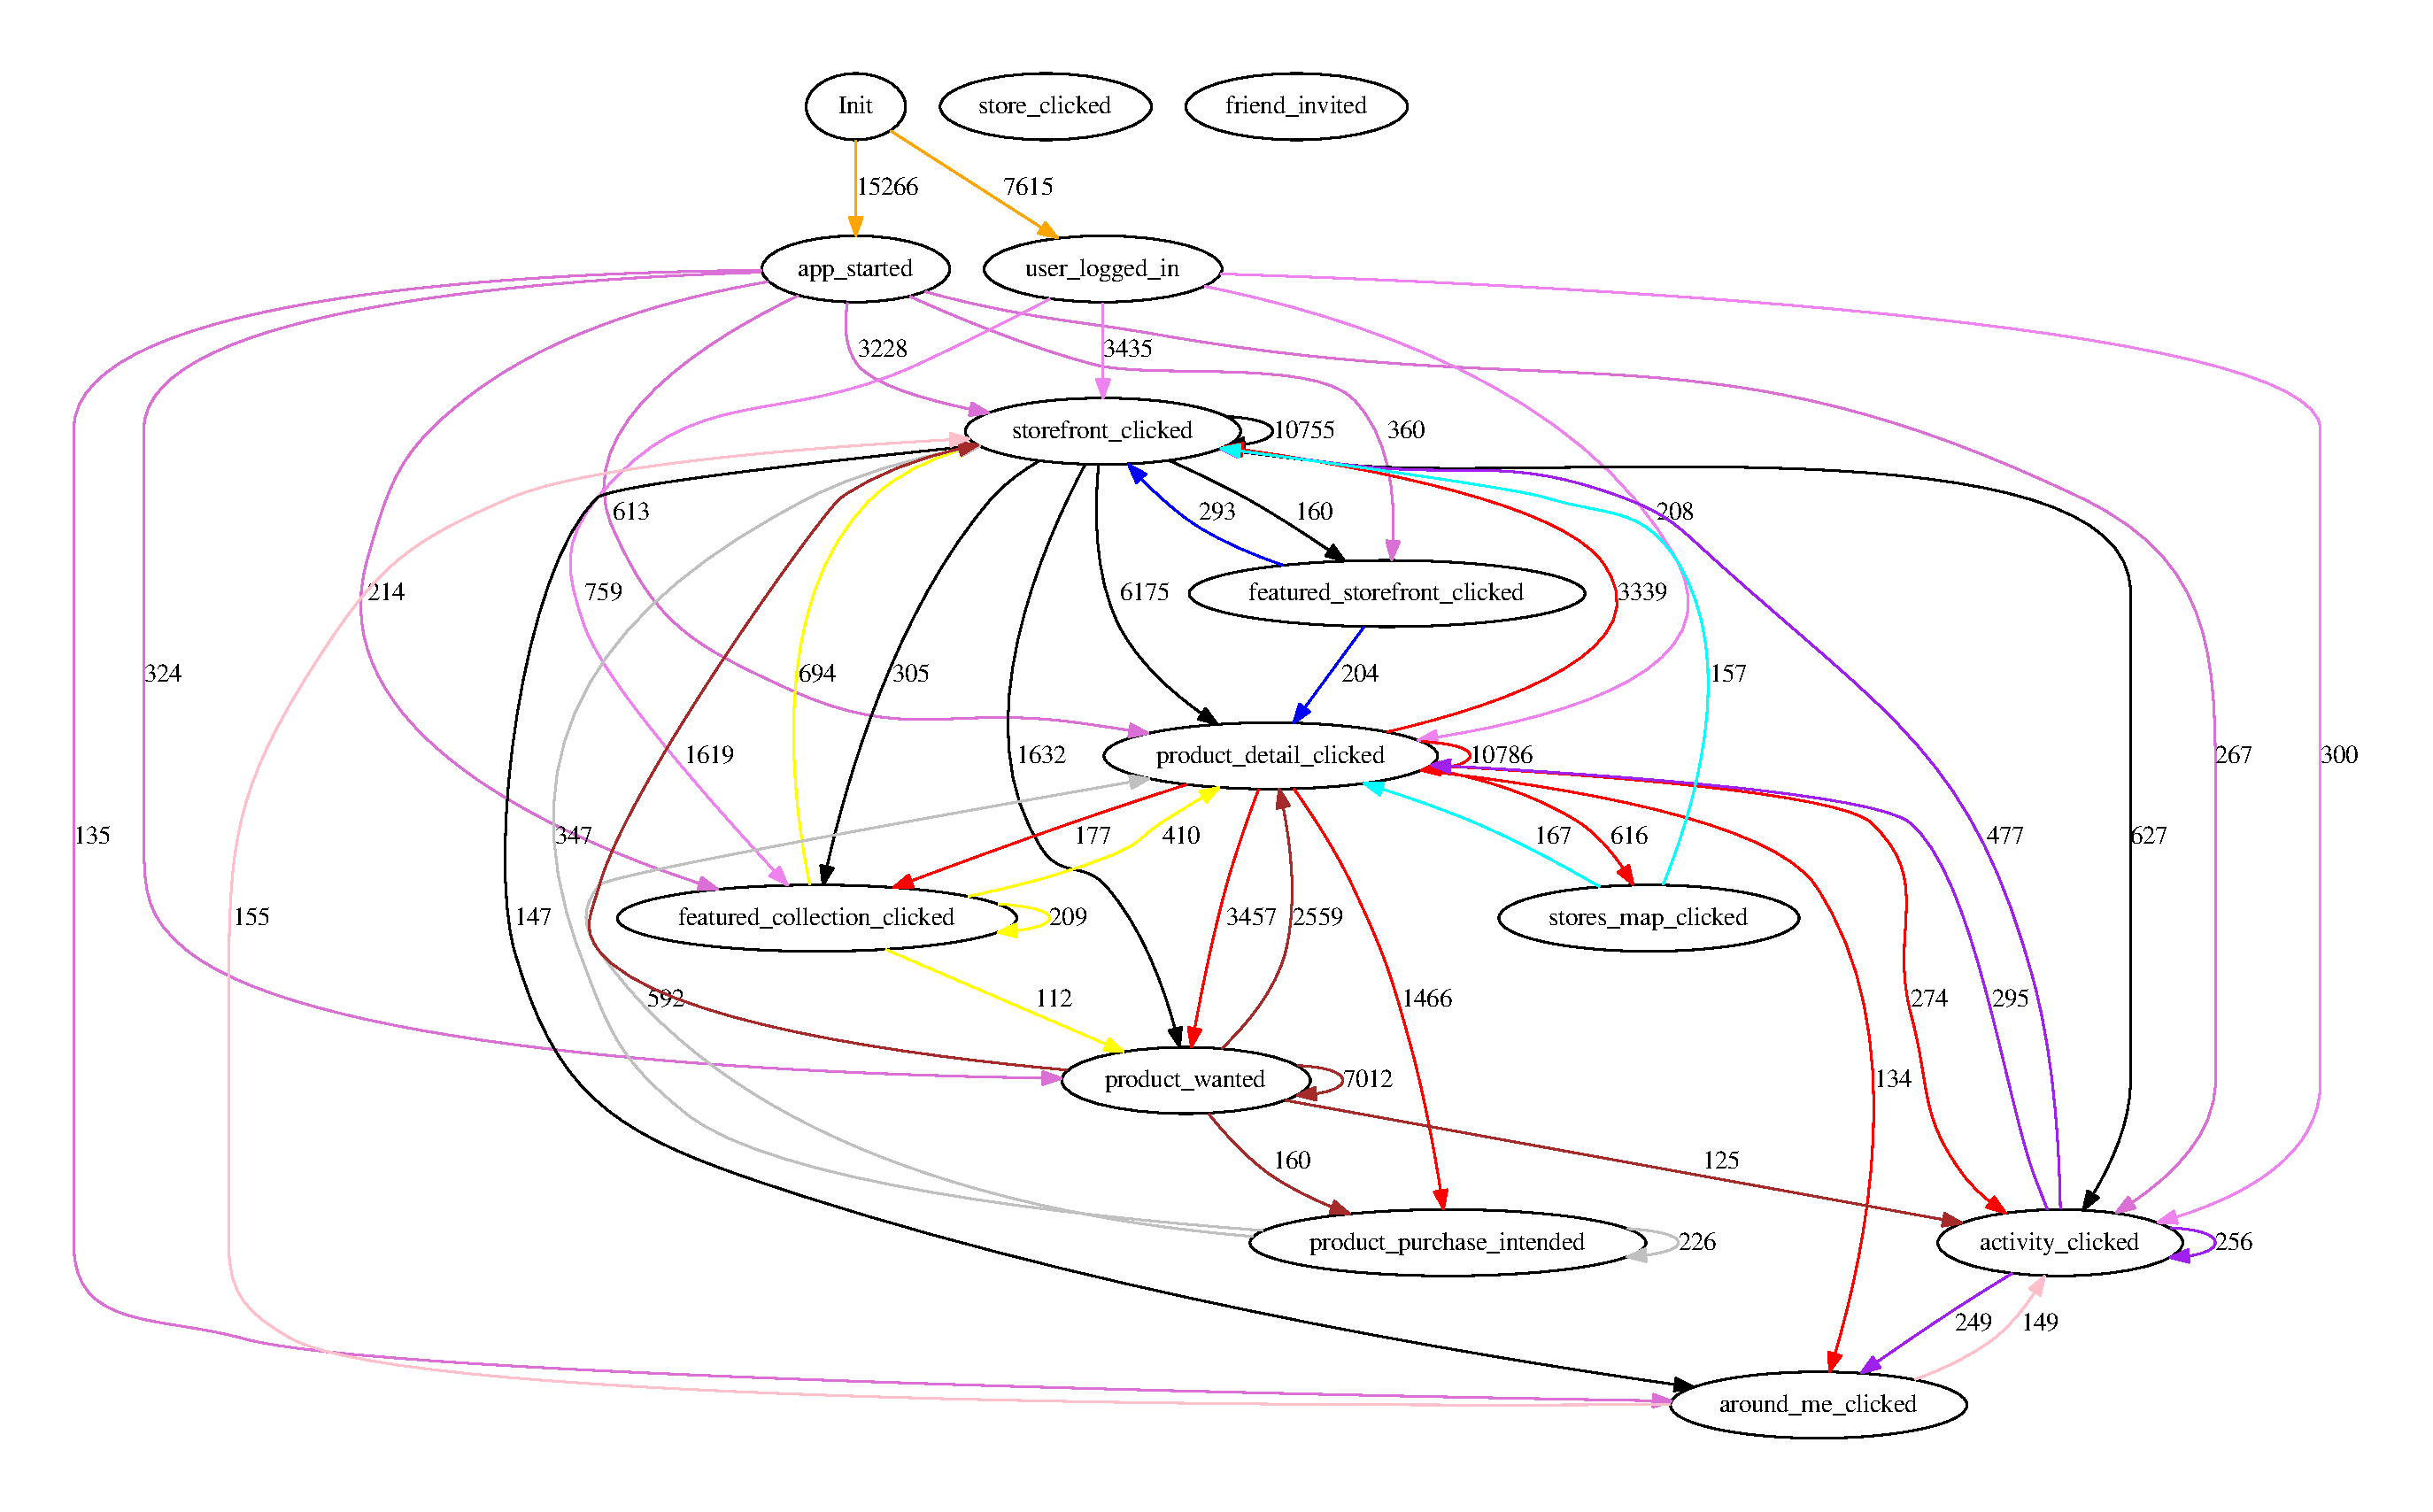
\includegraphics[width=5in]{image/statesInteractionFalse-gvfile.pdf}
        \centering
        \caption[States in session and how they interact]{The different states of the system and how they interact with each other.}
        \label{figure:statesInteractions}
    \end{figure}

\chapter{Extended State Of the Art}
\label{app:sota}

\section{Fashion domain}

\marginpar{TODO: Fix some kind of left align centering og content}
\begin{table}[H]
    \centering
    \begin{tabular}{ccc}
    \toprule
      \multicolumn{2}{c}{Concrete Attributes (Product Features)} & Abstract Attributes (Attitude-Based) \\
      \cmidrule(r{1em}){1-2}
      \multicolumn{1}{c}{Intrinsic (Hedonic)} & \multicolumn{1}{c}{Extrinsic} 				 	& \\ \midrule
      Style 				& Price						 	& Fun \\
      Color				& Brand 					 	& Entertainment \\
      Patten 				& Country of origin			 	& Enjoyment\\
      Fabric/fiber 		& Place(Store) 				 	& Need \\
      Appearance	   	 	& Salespeson's evaluation	 	&  Function\\
      Fashionability  	& Approval of others 		 	&\\
      Durability			& Coordination with wardrobe 	&\\
      Comfort				&								& \\
      Quality				&								& \\
      Fit					&								& \\
      Care 				&								& \\
    \bottomrule
    \end{tabular}
    \caption[Consumers' Purchase Decisions]{The attributes effecting the consumer when in the process of consuming products~\cite{dutton2006}}
    \label{table:ConsumersPurchaseDec}
\end{table}

\section{SoBazaar Competitors}\label{app:sec:soCompetitors}
\subsubsection{Flink} % (fold)
\label{par:flink}
    "Flink is THE brand-new app to discover, get inspired and share trendy looks from top fashion bloggers" - About Flink~\cite{flink}.

    Flink is a fashion discovery application for iPhone.
    It allows the user to browse fashion blogs, hot brands and new trends.

    The content displayed can be "liked" and can be a collection of clothes from different brands.
    If the user is interested in the item, the application can redirect the user to the web page where it is sold.
    \begin{table}[H]
            \centering
            \begin{tabularx}{\linewidth}{>{\parskip1ex}X@{\kern4\tabcolsep}>{\parskip1ex}X}
                \toprule
                \hfil\bfseries Strengths
                &
                \hfil\bfseries Weaknesses
                \\\cmidrule(r{3\tabcolsep}){1-1}\cmidrule(l{-\tabcolsep}){2-2}
                Can follow other users \par
                Connect with facebook \par
                Ability to add item to a \emph{want list} \par
                &
                No personalized recommendations \par
                \\\bottomrule
                \end{tabularx}
        \caption[Recommendation related strengths and weaknesses of Flink~\cite{flink}]{This table is the list of the recommendation related strengths and weaknesses of the mobile fashion application Flink~\cite{flink}}
        \label{table:iphoneAppFlink}
    \end{table}
  % todo - might be more, but can't explore the application since it is iOS 7 required
% paragraph flink (end)

\subsubsection{Motilo} % (fold)
\label{par:motilo}
    "Motilo was launched in 2011 to answer that perennial fashion dilemma all women face --- what shall I wear tonight?" - About Motilo~\cite{motilo}.

    Items on the web page are gathered by the Motilo stylists.
    This gives the page a fresh set of items for the user to select from.

    Motilo gives the user the ability to put together item sets through dragging and dropping the items into a "fashion dilemma", or simply like items.
    The user can ask friends, the Motilo community or the Motilo stylists about suggestions regarding what to wear.
    If the user wants to buy an item, Motilo redirects the user to the page which sells the item in question.

    \begin{table}[H]
    \centering
    \begin{tabularx}{\linewidth}{>{\parskip1ex}X@{\kern4\tabcolsep}>{\parskip1ex}X}
        \toprule
        \hfil\bfseries Strengths
        &
        \hfil\bfseries Weaknesses
            \\\cmidrule(r{3\tabcolsep}){1-1}\cmidrule(l{-\tabcolsep}){2-2}
            Connected with facebook \par
            Ability to add item to a "want list" \par
            A feed with the most trending item collections \par
            Ask Motilo stylists for suggestions \par
            &
            Manual/limited personalized recommendations \par
            \\\bottomrule
            \end{tabularx}
            \caption[Recommendation related strengths and weaknesses of Motilo~\cite{motilo}]{This table is the list of the recommendation related strengths and weaknesses of e-commerce fashion web site Motilo~\cite{motilo}}
            \label{table:ecommenreceMotilo}
        \end{table}
% paragraph motilo (end)


\subsubsection{ModCloth} % (fold)
\label{par:modcloth}
    "A top e-retailer of indie clothing, accessories, and decor, and provide an engaging shopping experience where you, our customer, can have a voice" - About ModCloth~\cite{modcloth}

    ModCloth focuses on giving what the community is looking for.
    The user is given the opportunity to both be the seller and the buyer.
    The item base is affected by the user trough voting.
    \begin{table}[H]
            \centering
            \begin{tabularx}{\linewidth}{>{\parskip1ex}X@{\kern4\tabcolsep}>{\parskip1ex}X}
                \toprule
                \hfil\bfseries Strengths
                &
                \hfil\bfseries Weaknesses
                \\\cmidrule(r{3\tabcolsep}){1-1}\cmidrule(l{-\tabcolsep}){2-2}
                Ability to add item to a "want list" \par
                A feed with the most popular items \par
                A feed with new items \par
                A list of similar items \par
                &
                No personalized recommendations \par
                \\ \bottomrule
        \end{tabularx}
        \caption[Recommendation related strengths and weaknesses of
        ModCloth~\cite{modcloth}]{This table is the list of the recommendation
        related strengths and weaknesses of e-commerce fashion web site
        ModCloth~\cite{modcloth}}
        \label{table:ecommenreceModCloth}
    \end{table}
% paragraph modcloth (end)

\subsubsection{UsTrendy} % (fold)
\label{par:ustrendy}
    "UsTrendy allows you to shop and discover one-of-a-kind fashions from all over the world." - About UsTrendy~\cite{UsTrendy}

    UsTrendy has a large item database of more than hundred thousand unique items.

    When the user is viewing an item, UsTrendy displays other items the user might like, which have common traits with the one the user is currently watching.
    The currently viewed item can be added to a sopping cart.
    \begin{table}[H]
                \centering
                \begin{tabularx}{\linewidth}{>{\parskip1ex}X@{\kern4\tabcolsep}>{\parskip1ex}X}
                    \toprule
                    \hfil\bfseries Strengths
                    &
                    \hfil\bfseries Weaknesses
                    \\\cmidrule(r{3\tabcolsep}){1-1}\cmidrule(l{-\tabcolsep}){2-2}
                  Ability to add item to a "want list" \par
                  A feed with the most popular items \par
                  A feed with new items \par
                  A list of similar items \par
                  &
                  No personalized recommendations \par
                \\ \bottomrule
        \end{tabularx}
        \caption[Recommendation related strengths and weaknesses of UsTrendy~\cite{UsTrendy}]{This table is the list of the recommendation related strengths and weaknesses of e-commerce fashion web site UsTrendy~\cite{UsTrendy}}
        \label{table:ecommenreceUsTrendy}
    \end{table}
% paragraph ustrendy (end)

\subsubsection{Polyvore} % (fold)
\label{par:polyvore}
    "Polyvore is a new way to discover and shop for things you love." - About Polyvore~\cite{polyvore}

    In Polyvore the user can put together sets of items and show them off to their friends and others.
    The items shown on Polyvore are gathered based on the community of Polyvore.

    When accessing an item the user is shown similar items to the one which is currently being watched.
    When the user want to purchase an item, the user is redirected to the page which sells the item.
    \begin{table}[H]
                \centering
                \begin{tabularx}{\linewidth}{>{\parskip1ex}X@{\kern4\tabcolsep}>{\parskip1ex}X}
                \toprule
                \hfil\bfseries Strengths
                &
                \hfil\bfseries Weaknesses
                \\\cmidrule(r{3\tabcolsep}){1-1}\cmidrule(l{-\tabcolsep}){2-2}
                    Ability to add item to a "want list" \par
                    The user can follow other users \par
                    Crawl other fashion sites to add to their item base \par
                    A feed with trending items \par
                    A list of recently viewed items \par
                &
                    No personalized recommendations \par
                \\ \bottomrule
        \end{tabularx}
        \caption[Recommendation related strengths and weaknesses of
        Polyvore~\cite{polyvore}]{This table is the list of the recommendation
        related strengths and weaknesses of e-commerce fashion web site
        Polyvore~\cite{polyvore}}
        \label{table:ecommenrecePolyvore}
    \end{table}
% paragraph polyvore (end)

\subsubsection{Clothia} % (fold)
\label{par:clothia}
    "An online destination where you can mix and match outfits, share looks you love, even try on clothes virtually via your webcam using augmented reality technology" - About Clothia~\cite{clothia}

    The user can put together a set of clothes from the web site and make a "set".
    The set can be shared with other users and like by other users.
    If the user is interested in buying an item, the user is redirected to the page from which the item is sold.
    \begin{table}[H]
                \centering
                \begin{tabularx}{\linewidth}{>{\parskip1ex}X@{\kern4\tabcolsep}>{\parskip1ex}X}
                \toprule
                \hfil\bfseries Strengths
                &
                \hfil\bfseries Weaknesses
                \\\cmidrule(r{3\tabcolsep}){1-1}\cmidrule(l{-\tabcolsep}){2-2}
                Ability to add item to a "want list" \par
                The user can follow other users \par
                A feed with trending items \par
                &
                Lack personalized recommendations \par
                \\ \bottomrule
        \end{tabularx}
        \caption[Recommendation related strengths and weaknesses of Clothia~\cite{clothia}]{This table is the list of the recommendation related strengths and weaknesses of e-commerce fashion web site Clothia~\cite{clothia}}
        \label{table:ecommenreceClothia}
    \end{table}
% paragraph clothia (end)

\subsubsection{Trendabl} % (fold)
\label{par:trendabl}
    "Trendabl is a community of people who love fashion" - About Trendable~\cite{trendabl}

    The user is shown a feed with the newest items, and is free to browse different sets of collections, such as collections with shoes and pants.
    If the user wants to buy an item it can be added to a shopping chart.
    \begin{table}[H]
                    \centering
                    \begin{tabularx}{\linewidth}{>{\parskip1ex}X@{\kern4\tabcolsep}>{\parskip1ex}X}
                    \toprule
                    \hfil\bfseries Strengths
                    &
                    \hfil\bfseries Weaknesses
                    \\\cmidrule(r{3\tabcolsep}){1-1}\cmidrule(l{-\tabcolsep}){2-2}
                    Ability to add item to a "want list" \par
                    The user can follow other users \par
                    System recommends the top users in the system for the user to follow \par
                    &
                    No personalized recommendations \par
                    \\ \bottomrule
        \end{tabularx}
        \caption[Recommendation related strengths and weaknesses of Trendabl~\cite{trendabl}]{This table is the list of the recommendation related strengths and weaknesses of e-commerce fashion web site Trendabl~\cite{trendabl}}
        \label{table:ecommenreceTrendabl}
    \end{table}
% paragraph trendabl (end)


\subsubsection{Rue La La} % (fold)
\label{par:rue_la_la}
    "Rue La La is the destination for the most desired brands" - About Rue La La~\cite{RueLaLa}

    Rue La La is a sale on site e-commerce web site.
    It is built up of a set of different boutiques, which can be browsed by the user.
    When the user is watching an item, Rue La La shows other items from the current boutique.

    \begin{table}[H]
                \centering
                \begin{tabularx}{\linewidth}{>{\parskip1ex}X@{\kern4\tabcolsep}>{\parskip1ex}X}
                \toprule
                \hfil\bfseries Strengths
                &
                \hfil\bfseries Weaknesses
                \\\cmidrule(r{3\tabcolsep}){1-1}\cmidrule(l{-\tabcolsep}){2-2}
                Ability to add item to a "want list" \par
                List of most popular items \par
                &
                No personalized recommendations \par
                \\ \bottomrule
        \end{tabularx}
        \caption[Recommendation related strengths and weaknesses of Rue La La~\cite{RueLaLa}]{This table is the list of the recommendation related strengths and weaknesses of e-commerce fashion web site Rue La La~\cite{RueLaLa}}
        \label{table:ecommenreceRueLaLa}
    \end{table}
% paragraph rue_la_la (end)

\subsubsection{Zalando} % (fold)
\label{par:zalando}
    "Clothes, accessories, sports items, beauty products" - About Zalando~\cite{Zalando}

    Zalando has a large set of items.
    When browsing an item the user is shown a set of similar items the user might also like, and a set of items which might "go well"  with the currently viewed item.

    \begin{table}[H]
                    \centering
                    \begin{tabularx}{\linewidth}{>{\parskip1ex}X@{\kern4\tabcolsep}>{\parskip1ex}X}
                    \toprule
                    \hfil\bfseries Strengths
                    &
                    \hfil\bfseries Weaknesses
                    \\\cmidrule(r{3\tabcolsep}){1-1}\cmidrule(l{-\tabcolsep}){2-2}
                    Ability to add item to a "want list" \par
                    Shop on site \par
                    Similar items \par
                    &
                    No personalized recommendations \par
                    \\ \bottomrule
        \end{tabularx}
        \caption[Recommendation related strengths and weaknesses of Zalando~\cite{Zalando}]{This table is the list of the recommendation related strengths and weaknesses of e-commerce fashion web site Zalando~\cite{Zalando}}
        \label{table:ecommenreceZalando}
    \end{table}
% paragraph zalando (end)

\subsubsection{Ellos~\cite{Ellos}} % (fold)
\label{par:ellos}
    Ellos is a e-commerce web site, which specializes in fashion.

    When browsing an item, similar items to the one currently being watched is presented to the user.
    Other items which might go well with the item is also presented for the user.

    \begin{table}[H]
                \centering
                \begin{tabularx}{\linewidth}{>{\parskip1ex}X@{\kern4\tabcolsep}>{\parskip1ex}X}
                \toprule
                \hfil\bfseries Strengths
                &
                \hfil\bfseries Weaknesses
                \\\cmidrule(r{3\tabcolsep}){1-1}\cmidrule(l{-\tabcolsep}){2-2}
                Ability to add item to a "want list" \par
                Shop on site \par
                Similar items \par
                On site most popular list \par
                Items which might go well with the current \par
                &
                No personalized recommendations \par
                \\ \bottomrule
        \end{tabularx}
        \caption[Recommendation related strengths and weaknesses of Ellos~\cite{Ellos}]{This table is the list of the recommendation related strengths and weaknesses of e-commerce fashion web site Ellos~\cite{Ellos}}
        \label{table:ecommenreceEllos}
    \end{table}
% paragraph ellos (end)

\subsubsection{LookBook} % (fold)
\label{par:lookbook}
    "LOOKBOOK is the \#1 source for fashion inspiration from real people around the world." - About LookBook~\cite{LookBook}

    LookBook is a leading online community which is centered around the looks of the users.
    The users can share their own looks and keep up with other users through watching their uploads.
    With over 1.2 million members LookBook is constantly up to date on the newest fashion trends.
    \begin{table}[H]
                \centering
                \begin{tabularx}{\linewidth}{>{\parskip1ex}X@{\kern4\tabcolsep}>{\parskip1ex}X}
                \toprule
                \hfil\bfseries Strengths
                &
                \hfil\bfseries Weaknesses
                \\\cmidrule(r{3\tabcolsep}){1-1}\cmidrule(l{-\tabcolsep}){2-2}
                Ability to add item to a "want list" \par
                Shop on site \par
                Similar items \par
                Most popular items list \par
                Hot items list \par
                &
                No personalized recommendations \par
                \\ \bottomrule
        \end{tabularx}
        \caption[Recommendation related strengths and weaknesses of LookBook~\cite{LookBook}]{This table is the list of the recommendation related strengths and weaknesses of e-commerce fashion web site LookBook~\cite{LookBook}}
        \label{table:ecommenreceLookBook}
    \end{table}
% paragraph lookbook (end)


\subsubsection{Fashiolista} % (fold)
\label{par:fashiolista}
    "Let Fashiolista's community be your style guide in the online fashion jungle" - About Fasho~\cite{Fashiolista}

    The items on Fashiolista is selected by the users of Fashiolista, and the sites is therefore customized to fit the user crowd's wishes and interests.

    When accessing an item, the user is presented with the item, and a set of other items from the store the current item originated from.
    Other users who liked the item are also shown, so the user can browse their personal want list.
    \begin{table}[H]
                    \centering
                    \begin{tabularx}{\linewidth}{>{\parskip1ex}X@{\kern4\tabcolsep}>{\parskip1ex}X}
                    \toprule
                    \hfil\bfseries Strengths
                    &
                    \hfil\bfseries Weaknesses
                    \\\cmidrule(r{3\tabcolsep}){1-1}\cmidrule(l{-\tabcolsep}){2-2}
                Ability to add item to a "want list" \par
                On site most popular list \par
             &
                 No personalized recommendations \par
             \\ \bottomrule
        \end{tabularx}
        \caption[Recommendation related strengths and weaknesses of Fashiolista~\cite{Fashiolista}]{This table is the list of the recommendation related strengths and weaknesses of e-commerce fashion web site Fashiolista~\cite{Fashiolista}}
        \label{table:ecommenreceFahiolista}
    \end{table}
% paragraph fashiolista (end)

\subsubsection{ShopStyle} % (fold)
\label{par:shopstyle}
    "POPSUGAR is a global women's lifestyle brand focused in media, commerce, and technology" - About ShopStyle~\cite{ShopStyle}

    ShopStyle is a commerce brand of POPSUGAR.
    ShopStyle displays items from other e-commerce web sites, and redirects the user directly to the e-commerce web site from which the item clicked originated.
    Items can be liked on ShopStyle, and viewed in less detail at the web page of ShopStyle.
    \begin{table}[H]
                    \centering
                    \begin{tabularx}{\linewidth}{>{\parskip1ex}X@{\kern4\tabcolsep}>{\parskip1ex}X}
                    \toprule
                    \hfil\bfseries Strengths
                    &
                    \hfil\bfseries Weaknesses
                    \\\cmidrule(r{3\tabcolsep}){1-1}\cmidrule(l{-\tabcolsep}){2-2}
                Ability to add item to a "want list" \par
                Similar items \par
                Editor's picks \par
            &
                No personalized recommendations \par
            \\ \bottomrule
        \end{tabularx}
        \caption[Recommendation related strengths and weaknesses of ShopStyle~\cite{ShopStyle}]{This table is the list of the recommendation related strengths and weaknesses of e-commerce fashion web site ShopStyle~\cite{ShopStyle}}
        \label{table:ecommenreceShopStyle}
    \end{table}
% paragraph shopstyle (end)

\section{State of the Art: Evaluation}
\label{appendix:evaluation-metrics}

% Describe why this is in the Appendix.
In this section we will cover an in-depth study of evaluation metrics and
methods, which were not included in~\ref{sec:evaluation} as they are not
directly suited for either the domain or setting in the proposed system.
They are included here as they may provide clarity on \textit{why} they are not
suited, as well the fact that non-suitednes is a result in itself. Finally we
identify some resources of which the avid reader may do further research into
the field of evaluation recommender systems.

% Boostrapping in Appendix, as we do not use it and Helge proposed it.
\subsubsection{Using bootstrapping for validating offline experiments}
Bootstrapping~\cite{efron1994introduction} is used to estimate properties of an
estimate, such as bias, variance, confidence, intervals and prediction error.
This is done trough measuring these properties when sampling from an
approximated distribution, creating an empirical distribution of the observed
data.  Since the entire population is unknown it will not be possible to
calculate the true error from the sample data.  The idea then is that with this
information from sample data it is possible to say something about the
population.  Since it will not be possible to perform inference on:

\emph{sample data} $\rightarrow$ \emph{population} this is modeled as:
\emph{re-sample data} $\rightarrow$ \emph{sample data}.
The \emph{re-sample data} is a re-sampling of the sample data.

In practice an example to bootstrapping is when we want to calculate the
average height of the population worldwide.  The issue here is that it is not
as doable to measure everyone, so a subset of the population is used.  Since
the average on this number only will be an estimate of the actual world wide
average a sense of error margin must be introduced.  Bootstrapping is then used
to reduce the error of margin through re-sampling the sample data a large
number of times~\footnote{Numbers vary on sample size, but is often 1 000 to 10
000}, and new averages are calculated.  With these averages a histogram can be
produced, which provides an estimate of the distribution of this average.

\begin{figure}[H]
    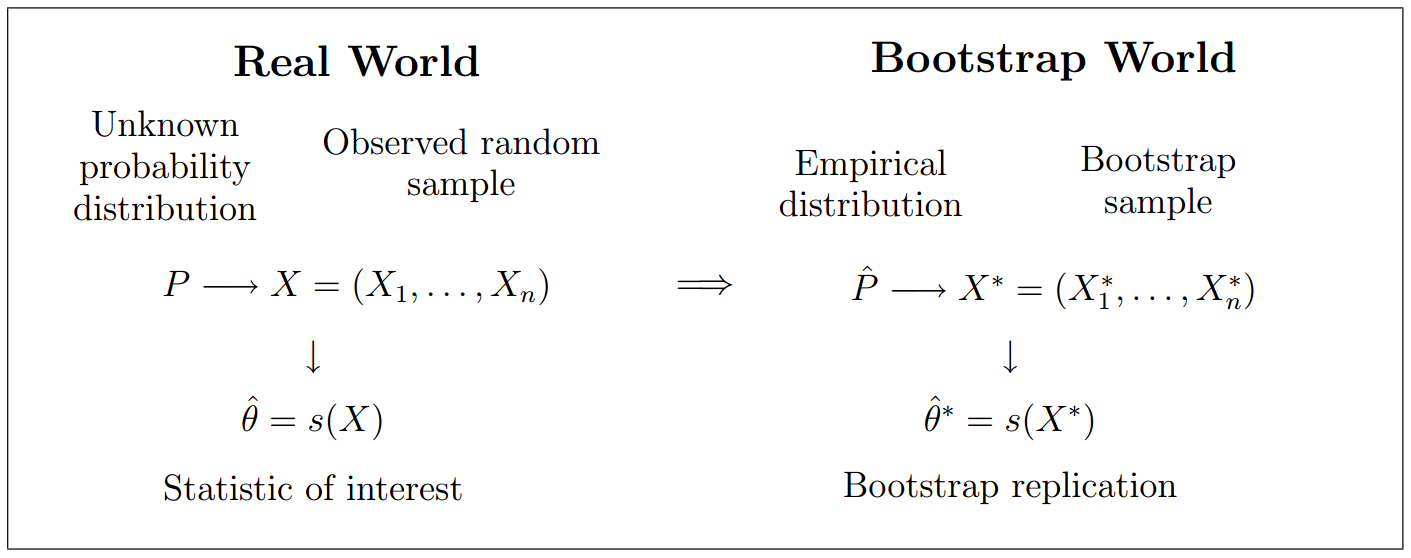
\includegraphics[scale=0.6]{image/bootstrap.png}
    \centering
    \caption[Bootstrapping principles]{A figure of the principles bootstrapping. Taken from~\cite{Eichler2003}}
    \label{figure:bootstrapping}
\end{figure}

One prominent issue with bootstrapping is that important properties of the
actual data might not be caught when undertaking the bootstrapping analysis
~\footnote{"Bootstrapping" comes from the phrase, "to pull oneself up by one's
bootstraps"~\cite{bootstrapSaying1843}}.

% Sub-section on resources available for avid readers who want further research
% into the field of evaluating recommender systems.
\subsubsection{Datasets for Offline Evaluation}
The main aim of a recommender system is to identify the set of items in a
dataset that might be interesting to a user based on their expressed
preferences. For a fashion recommender this would mean estimating how much a
user might like an item, by e.g.\\ predicting what rating a user might give an
item. In recent years, various test collections for different domains such as
books, music, movies have been made available to the public. These datasets
usually consist of user ratings similar to the ones used in this thesis (see
Section~\ref{}):

\begin{table}[H]
\centering
	\begin{tabular}{*{4}l}
	\toprule
		User ID & Item ID & Rating & Timestamp \\ \midrule
		1		  &	11	  &	5	    &  2014-12-15 10:14:51  \\
		2		  &	19	  &	2	    &  2014-12-12 11:44:31  \\
		\dots &	\dots &	\dots &  \dots                \\
	\bottomrule
	\end{tabular}
\caption{Classical recommender system dataset}
\end{table}

In recent years more or more datasets have been made available which contains
additional information such as demographic information about the users,
trust-networks, user-assigned tags and etc. Below we have listed a few selected
popular datasets containing additional information:

\begin{itemize}

\item \textbf{MovieLens 100k dataset}~\cite{Movielens}: The movielens dataset
	incorporates demographic information about the user in addition the
	traditional rating matrix

\item \textbf{Epinions dataset}~\cite{Epinions}: The Epinions dataset includes a
	trust-network, which specifices who-trust-whom in a social network based on
	customer reviews for the website Epinions.com

\item \textbf{The Million Song Dataset}~\cite{Bertin-Mahieux2011}: The million song
	dataset is a implicit feedback dataset. This data also includes information on the users,
	and audio features and song meta-data.

\item \textbf{The Book-Crossing Dataset}: The bookcrossing dataset consists of both implicit and explicit feedback,
	demographic information about users and some content based information about the books.
\end{itemize}

\chapter{Extended Implementation}
\label{app:impl}

\section{Implemented Functional Requirements}
\begin{enumerate}[label=\bfseries FR \arabic*:]
  \item {\color{ForestGreen}Blablaba}
  \item {\color{RedOrange}\st{Blablaba}}
\end{enumerate}

\section{Implemented Non Functional Requirements}
\begin{enumerate}[label=\bfseries NFR \arabic*:]
  \item {\color{ForestGreen}Blablaba}
  \item {\color{RedOrange}\st{Blablaba}}
\end{enumerate}

\section{Experimental Results}
\label{app:results}


%----------------------------------------------
% BIBLIOGRAPHY
%----------------------------------------------
\clearpage
\addcontentsline{toc}{chapter}{References}
\bibliographystyle{plain}
\bibliography{references}

\end{document}
